\section{Introduzione} 
Questa è l'introduzione.
\subsection{L'azienda}
\begin{figure}[htbp]
\begin{center}
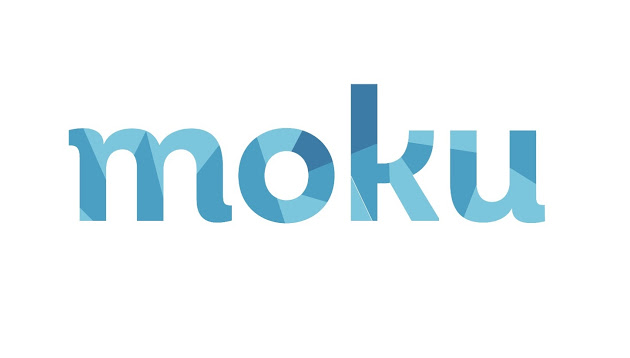
\includegraphics[height=4cm]{Pics/logo_moku.jpg}
\end{center}
\end{figure}
Moku S.r.l è una startup nata nel 2013 e situata in H-Farm. 
Il lavoro è organizzato seguendo il modello agile Scrum supportato dalla suite Atlassian che offre un servizio cloud per la gestione dei compiti e dei progetti.
L'azienda lavora a stretto contatto con il cliente definendo requisiti, user experience dei prodotti realizzati ed opportunità di business.
Obiettivo primario dell'azienda è la qualità del software e l'utilizzo di tecnologie recenti poiché l'alto coefficiente innovativo dei prodotti realizzati rende necessaria una costante manutenzione che si vuole sia il più agevole possibile.

\subsubsection{Origine}
Il nome della startup, in hawaiiano, significa \textit{isola}. Questo perché l'idea iniziale era una applicazione web per studenti dove un \textit{"moku"} era visto come uno spazio personale (un’isola), ma allo stesso tempo uno spazio di collaborazione, rappresentando un \textit{arcipelago} di isole collegate tra loro.
In origine si basava sulla realizzazione di una applicazione il cui uso era riservato principalmente agli studenti. Ad ogni utente era data la possibilità di caricare i propri documenti in diverse tipologie di formato. Una volta aperti, era possibile prendere degli appunti su un layer posto sopra al documento caricato. Questo può essere condiviso con i propri collaboratori. Era anche possibile registrare la lezione e mettere delle note anche alla traccia audio, la quale si poteva sincronizzare con un particolare documento.
\subsubsection{Evoluzione}
Ora le attività dell'azienda si concentrano nella consulenza IT, in particolare nella realizzazione di software innovativo a supporto delle esigenze concrete dei clienti.
\subsection{Il progetto di Stage}
Moku	Srl	in	collaborazione	con	professionisti	del	settore,	ha	sviluppato	un	software	web	based che	

supporta	le	aziende	che	intendono	avvalersi	dell’asseverazione	in	ambito	della	sicurezza	sul	lavoro.	

Dal	 punto	 di	 vista	 tecnico	 utilizza	 un	 sistema	 esperto	 per	mappare	 le	 norme	 in	 tema	 di	 sicurezza,	

individuare	 i	 punti	 deboli	 dell’azienda,	 ricordare	 al	 responsabile	 le	 scadenze	 e	 conservare	 ed	

indicizzare	il	patrimonio	documentale	dell’azienda	in	ambito	sicurezza.

Il	 sistema	 ha	 un	 funzione	 proattiva	 e	 dinamica,	 variando	 gli	 allarmi	 in	 base	 alla	 variazione	 delle	

norme	 e	 allo	 stato	 dell’azienda	 (es.	 al	 crescere	 o	 diminuire	 del	 numero	 dei	 dipendenti,	 al	 variare	

della	 superficie	 delle	 sedi	 aziendali,	 dei	 cantieri...).

La	 webapp	 si	 comporta	 quindi	 come	 un	 consulente	 digitale	 per	 l’azienda	 aiutandola	 a	 mantenere	

aggiornato	il	suo	modello	di	sicurezza	e	a	rispettarlo.

Questo	le	permette	all’azienda	asseverata	di	accedere	a	significativi	premi	INAIL,	di	ottenere	punti	in	

graduatoria	 in	 bandi	 pubblici	 e	 di	 sollevare	 il	 datore	 di	 lavoro	 da	 responsabilità	 penali	 in	 caso	 di	

infortuni	legati	ad	una	mala	gestione	della	sicurezza.